%
%                  Politecnico di Milano
%
%          Gruppo: AM34
%            A.A.: 2022/2023
%
% Ultima modifica: 22/04/2023
%
%     Descrizione: Prova Finale (Progetto) di Ingegneria del Software - A.A. 2022/23
%                  Documento di specifica del protocollo di comunicazione
%

\documentclass[a4paper,11pt]{article} % tipo di documento
\usepackage[T1]{fontenc} % codifica dei font
\usepackage[utf8]{inputenc} % lettere accentate da tastiera
\usepackage[english,italian]{babel} % lingua del documento
\usepackage{lipsum} % genera testo fittizio
\usepackage{url} % per scrivere gli indirizzi Internet e/o di riferimento nella pagina

\usepackage[hidelinks]{hyperref} % per modificare il comportamento dei collegamenti ipertestuali (+ leva colore attorno)

\usepackage[margin=0.7in]{geometry} % margine di pagina

\usepackage{graphicx} % per inserire immagini

\usepackage[outputdir=../auxil]{minted} % per colorazione automatica del codice
% \usepackage{pythonhighlight} % per Python

\setminted{ % si può impostare il linguaggio specifico con \setminted[JSON] ad esempio
%    linenos=true,
    breaklines=true,
    encoding=utf8,
    fontsize=\normalsize,
%    frame=lines
}

\setminted[Java]{ % si può impostare il linguaggio specifico con \setminted[JSON] ad esempio
    linenos=true,
    breaklines=true,
    encoding=utf8,
    fontsize=\normalsize,
    frame=lines
}

\makeatletter % rimuove contorno rosso quando rilevati errori di Pygments
\AtBeginEnvironment{minted}{\dontdofcolorbox}
\def\dontdofcolorbox{\renewcommand\fcolorbox[4][]{##4}}
\makeatother

\usepackage{fancyhdr} % per gestione intestazione e piè di pagina

\hypersetup{ % metadati di titolo e autore nel PDF
    pdftitle={Prova Finale di Ingegneria del Software - A.A. 2022/23},
    pdfauthor={Andrea Caravano - Biagio Cancelliere - Alessandro Cavallo - Allegra Chiavacci}
}

\setlength{\parindent}{0pt} % rimuove l'indentazione del testo

\begin{document}
    \pagestyle{fancy}
    \fancyhead{}\fancyfoot{}
    \fancyhead[L]{\textbf{Prova Finale (Progetto) di Ingegneria del Software - A.A. 2022/23}}
    \fancyhead[R]{Gruppo AM34}
    \fancyfoot[C]{\thepage}

    \author{Andrea Caravano \and Biagio Cancelliere \and Alessandro Cavallo \and Allegra Chiavacci}
    \title{\textbf{\Large{Prova Finale (Progetto) di Ingegneria del Software - A.A. 2022/23\\Documento di specifica del protocollo di comunicazione}}}
    \maketitle

    \tableofcontents

    \newpage


    \section{Socket}\label{sec:socket}
    L'architettura prevede l'uso di un eseguibile Client e di uno Server.

    \smallskip
    Sono inoltre state formulate delle entità puramente descrittive, al fine di serializzare e deserializzare strutture parziali, semplificate per il solo client.

    \subsection*{Messaggi di stato}

    I messaggi di stato rappresentano la forma degli scambi relativi all'evoluzione delle fasi del gioco,
    delle sue mosse e della loro formalizzazione e verifica di correttezza generale.

    \smallskip

    \textbf{Nota bene}: al fine di facilitarne la lettura, gli scambi di messaggi presentati nel seguito sono scritti su più righe.
    In fase di implementazione, questi vengono inviati su una sola riga, in formato JSON.

    \smallskip
    Sono definiti i messaggi seguenti.

    \subsection{Accesso al gioco}\label{subsec:accesso-al-gioco}

    \subsubsection{Identificativo del gioco}
    Scambio dell'identificativo del gioco di cui il client desidera entrare a far parte.

    \paragraph{Formalizzazione}
    \begin{minted}{JSON}
{
  "status": "Sending_Identifier",
  "message": "Game's name"
}
    \end{minted}
    Dove \textsf{Game's name} rappresenta il nome del gioco di cui il client desidera di entrare a far parte.

    \subsubsection{Numero di giocatori}
    Scambio del numero di giocatori di una nuova partita.
    Il messaggio è per sua natura opzionale.

    \paragraph{Richiesta}
    \begin{minted}{JSON}
{
  "status": "Request_NumberOfPlayers"
}
    \end{minted}

    \paragraph{Risposta}
    \begin{minted}{JSON}
{
  "status": "Response_NumberOfPlayers",
  "message": "4"
}
    \end{minted}

    \newpage

    \subsubsection{Nickname}
    Scambio del nickname che il client vuole adottare nella partita.

    \paragraph{Richiesta}
    \begin{minted}{JSON}
{
  "status": "Request_Nickname"
}
    \end{minted}

    \paragraph{Risposta}
    \begin{minted}{JSON}
{
  "status": "Response_Nickname",
  "message": "Player3"
}
    \end{minted}
    Dove \textsf{Player3} rappresenta il nickname che il giocatore vuole adottare all'interno della partita.

    \subsubsection{Richiesta negata}
    La richiesta di ammissione alla partita non è stata accettata.
    Rivedere l'integrità dei parametri trasmessi.

    \paragraph{Formalizzazione}
    \begin{minted}{JSON}
{
  "status": "Denied_Request",
  "message": "Nickname is already in use"
}
    \end{minted}

    Dove è stata motivata la negata accettazione.

    \subsubsection{Richiesta accettata}
    La richiesta di ammissione alla partita è stata accettata.

    \paragraph{Formalizzazione}
    \begin{minted}{JSON}
{
  "status": "Accepted_Request"
}
    \end{minted}

    \newpage

    \subsection{Gestione del turno}\label{subsec:gestione-del-turno}

    \subsubsection{Non è il tuo turno}
    Il client non è il giocatore corrente.

    Esso attende l'evoluzione del gioco e viene informato dei cambiamenti in atto, in seguito alle mosse degli altri giocatori.

    \paragraph{Formalizzazione}
    \begin{minted}{JSON}
{
  "status": "NotYourTurn"
}
    \end{minted}

    \subsubsection{Mossa}
    Messaggio di formalizzazione di una mossa del giocatore corrente.

    \paragraph{È il tuo turno}
    Il giocatore corrente riceve l'indicazione di poter procedere con una richiesta di mossa, a cui il server risponde.
    \begin{minted}{JSON}
{
  "status": "YourTurn"
}
    \end{minted}

    \paragraph{Richiesta}
    \begin{minted}{JSON}
{
  "status": "Move_Request",
  "message": "{
                "column": 1,
                "x": [
                        3,
                        3,
                        3
                     ],
                "y": [
                        3,
                        4,
                        2
                      ]
              }"
}
    \end{minted}

    Dove sono indicate (in forma di lista) le singole/coppie/triplette di coordinate facenti parte della mossa corrente.

    Nell'esempio, si sta indicando la volontà di prendere dalla plancia di gioco le carte oggetto nella riga 3,
    colonne 2, 3, 4 e di inserirle nella propria libreria alla colonna 1.

    Si noti che l'ordine delle coordinate (che in questo caso differiscono solo per la coordinata $y$) è vincolante, relativamente
    all'inserimento nella libreria del giocatore.

    \newpage

    \subsubsection{Mossa andata a buon fine}
    La mossa richiesta è andata a buon fine.

    \paragraph{Formalizzazione}
    \begin{minted}{JSON}
{
  "status": "SuccessfulMove"
}
    \end{minted}

    \subsubsection{Mossa invalida}
    La mossa richiesta era invalida e non è stata eseguita.

    \paragraph{Formalizzazione}
    \begin{minted}{JSON}
{
  "status": "FailedMove"
}
    \end{minted}

    \subsubsection{Ultimo turno}
    Messaggio broadcast inviato a tutti i client, una volta completata una mossa.

    Il turno corrente viene ultimato, chi ha già eseguito la propria mossa ha concluso la partita.

    \paragraph{Formalizzazione}
    \begin{minted}{JSON}
{
  "status": "LastTurn"
}
    \end{minted}

    \subsubsection{Mossa permessa}
    A seguire il messaggio di ultimo turno, il server informa il giocatore sulla possibilità di dover concludere l'ultimo turno con un'altra mossa o meno.

    Il messaggio sarà seguito da un ordinario scambio caratterizzante un turno di gioco.

    \paragraph{Formalizzazione}
    \begin{minted}{JSON}
{
  "status": "MoveAllowed"
}
    \end{minted}

    \subsubsection{Mossa non permessa}
    A seguire il messaggio di ultimo turno, il server informa il giocatore sulla possibilità di dover concludere l'ultimo turno con un'altra mossa o meno.

    Il giocatore si trovava dunque in una posizione precedente al giocatore che ha ottenuto la carta di fine gioco.

    \paragraph{Formalizzazione}
    \begin{minted}{JSON}
{
  "status": "MoveNotAllowed"
}
    \end{minted}

    \newpage

    \subsubsection{La partita è finita}
    Alla conclusione dell'ultimo turno, il messaggio informa i client sulla fine del gioco.

    \paragraph{Formalizzazione}
    \begin{minted}{JSON}
{
  "status": "GameEnded"
}
    \end{minted}

    \subsubsection{Conclusione forzata}
    Un giocatore si è disconnesso, i client vengono informati di dover concludere forzatamente la partita.

    \paragraph{Formalizzazione}
    \begin{minted}{JSON}
{
  "status": "ForcedGameEnd"
}
    \end{minted}

    \newpage

    \subsection{Carattere generale}\label{subsec:carattere-generale}

    \subsubsection{Fine di sequenza}

    Messaggio che identifica la fine di una sequenza di linee di lunghezza arbitraria.

    \paragraph{Formalizzazione}

    \begin{minted}{JSON}
{
  "status": "EOS"
}
    \end{minted}

    \subsubsection{Invio della plancia di gioco}
    Viene allegata al messaggio la serializzazione JSON della plancia di gioco.

    Il client fa uso di un modello ridotto utile alla sola visualizzazione a video.

    \paragraph{Formalizzazione}
    \begin{minted}{JSON}
{
  "status": "SendingBoard",
  "message": "{
  "spaces": [
    [
      {
        "x": 0,
        "y": 0,
        "usable": false,
        "card": [
          null
        ],
        "dots": [
          null
        ]
      },
        ...
        {
        "x": 2,
        "y": 3,
        "usable": true,
        "card": [
          {
            "type": "GAMES",
            "image": 2
          }
        ],
        "dots": [
          null
        ]
      },
        ...
    }
  ]
  }"
}
    \end{minted}

    Dove sono stati mostrati due spazi di una plancia di gioco esemplificativa.

    \subsubsection{Invio della libreria personale}
    Viene allegata al messaggio la serializzazione JSON della libreria personale del giocatore.

    Il client fa uso di un modello ridotto utile alla sola visualizzazione a video.

    \paragraph{Formalizzazione}
    \begin{minted}{JSON}
{
  "status": "SendingShelf",
  "message": "{
  "cards": [
    [
      [
        {
          "type": "CATS",
          "image": 2
        }
      ],
      [
        {
          "type": "BOOKS",
          "image": 3
        }
      ],
        ...
    ]
  ]
  }"
}
    \end{minted}

    Dove sono state mostrate due celle di una libreria personale esemplificativa.

    \subsubsection{Invio della carta obiettivo personale}
    Viene allegata al messaggio la serializzazione JSON della propria carta obiettivo personale.

    Il client fa uso di un modello ridotto utile alla sola visualizzazione a video.

    \paragraph{Formalizzazione}
    \begin{minted}{JSON}
{
  "status": "SendingPersonalGoalCard",
  "message": "{
  "type": 1,
  "pattern": [
    [
      [
        "PLANTS"
      ],
      [
        null
      ],
      [
        "FRAMES"
      ],
      [
        null
      ],
      [
        null
      ]
    ],
    ...
  ]
  }"
}
    \end{minted}

    Dove è stata utilizzata come esempio la Carta obiettivo personale n. 1 (in riferimento all'ordinamento delle risorse fornite dal produttore).

    \subsubsection{Specifica della carta obiettivo comune}
    Viene allegata al messaggio la specifica della prima/seconda carta obiettivo comune.

    Il client fa uso di un modello ridotto utile alla sola visualizzazione a video.

    \paragraph{Formalizzazione}
    \begin{minted}{JSON}
{
  "status": "SendingCommonGoalCardSpecification",
  "message": "{
  "type": 5,
  "description": "Three columns each formed by 6 cards of maximum three different types. One column can show a different combination of another column."
  }"
}
    \end{minted}

    Dove è stata utilizzata come esempio la Carta obiettivo comune n. 5 (in riferimento all'ordinamento delle risorse fornite dal produttore).

    \subsubsection{Invio della classifica finale}
    Viene allegata al messaggio la serializzazione JSON della classifica finale.

    Il client fa uso di un modello ridotto utile alla sola visualizzazione a video.

    \paragraph{Formalizzazione}
    \begin{minted}{JSON}
{
  "status": "FinalScoreboard",
  "message": "{
  "scoreBoard": {
    "Player 4": 40,
    "Player 3": 30,
    "Player 2": 20,
    "Player 1": 10
  }
  }"
}
    \end{minted}

    \newpage

    \subsubsection{Stato non valido}
    Stato di default.

    \paragraph{Formalizzazione}
    \begin{minted}{JSON}
{
  "status": "InvalidStatus"
}
    \end{minted}

    \subsubsection{Errore}
    Errore, tipicamente generato da un'eccezione.

    \paragraph{Formalizzazione}
    \begin{minted}{JSON}
{
  "status": "Error",
  "message": "Reason of the error"
}
    \end{minted}
    Dove \textsf{Reason of the error} è la ragione dell'errore, comunicata dal server sottoforma di messaggio testuale.

    \subsection{Note conclusive}\label{subsec:note-conclusive}
    L'uso di strutture semplificate, lato client, obbliga a dover completare la struttura di informazioni che per sua natura il client non deve conoscere,
    quali i riferimenti alla plancia di gioco, alla libreria e alle carte di gioco.

    Ciò avviene attraverso l'uso di classi \texttt{Serializers}, che hanno il compito di identificare tali parametri e completarli con i riferimenti
    che il server fornisce, ottenendo la struttura completa.

    Ad esempio: in una mossa, il client comunica al server solo le coordinate da cui vuole prendere un gruppo di carte oggetto e la colonna in cui vuole posizionarle
    all'interno della propria libreria.

    Il server, per completare tale mossa, dovrà essere a conoscenza dei riferimenti di plancia di gioco e libreria, che verranno completati all'atto della
    deserializzazione.

    \smallskip

    I tipi di dato \texttt{Optional} inoltre, essendo di recente introduzione, hanno difficoltà ad essere correttamente serializzati (anche in RMI).

    Anche questo problema è risolto da classi appositamente costruite di \texttt{Serializers} e \texttt{Deserializers}.

    \newpage

    \subsection{Diagrammi di sequenza}\label{subsec:diagrammi-di-sequenza}

    \subsubsection{Accesso, selezione e ammissione al gioco}

    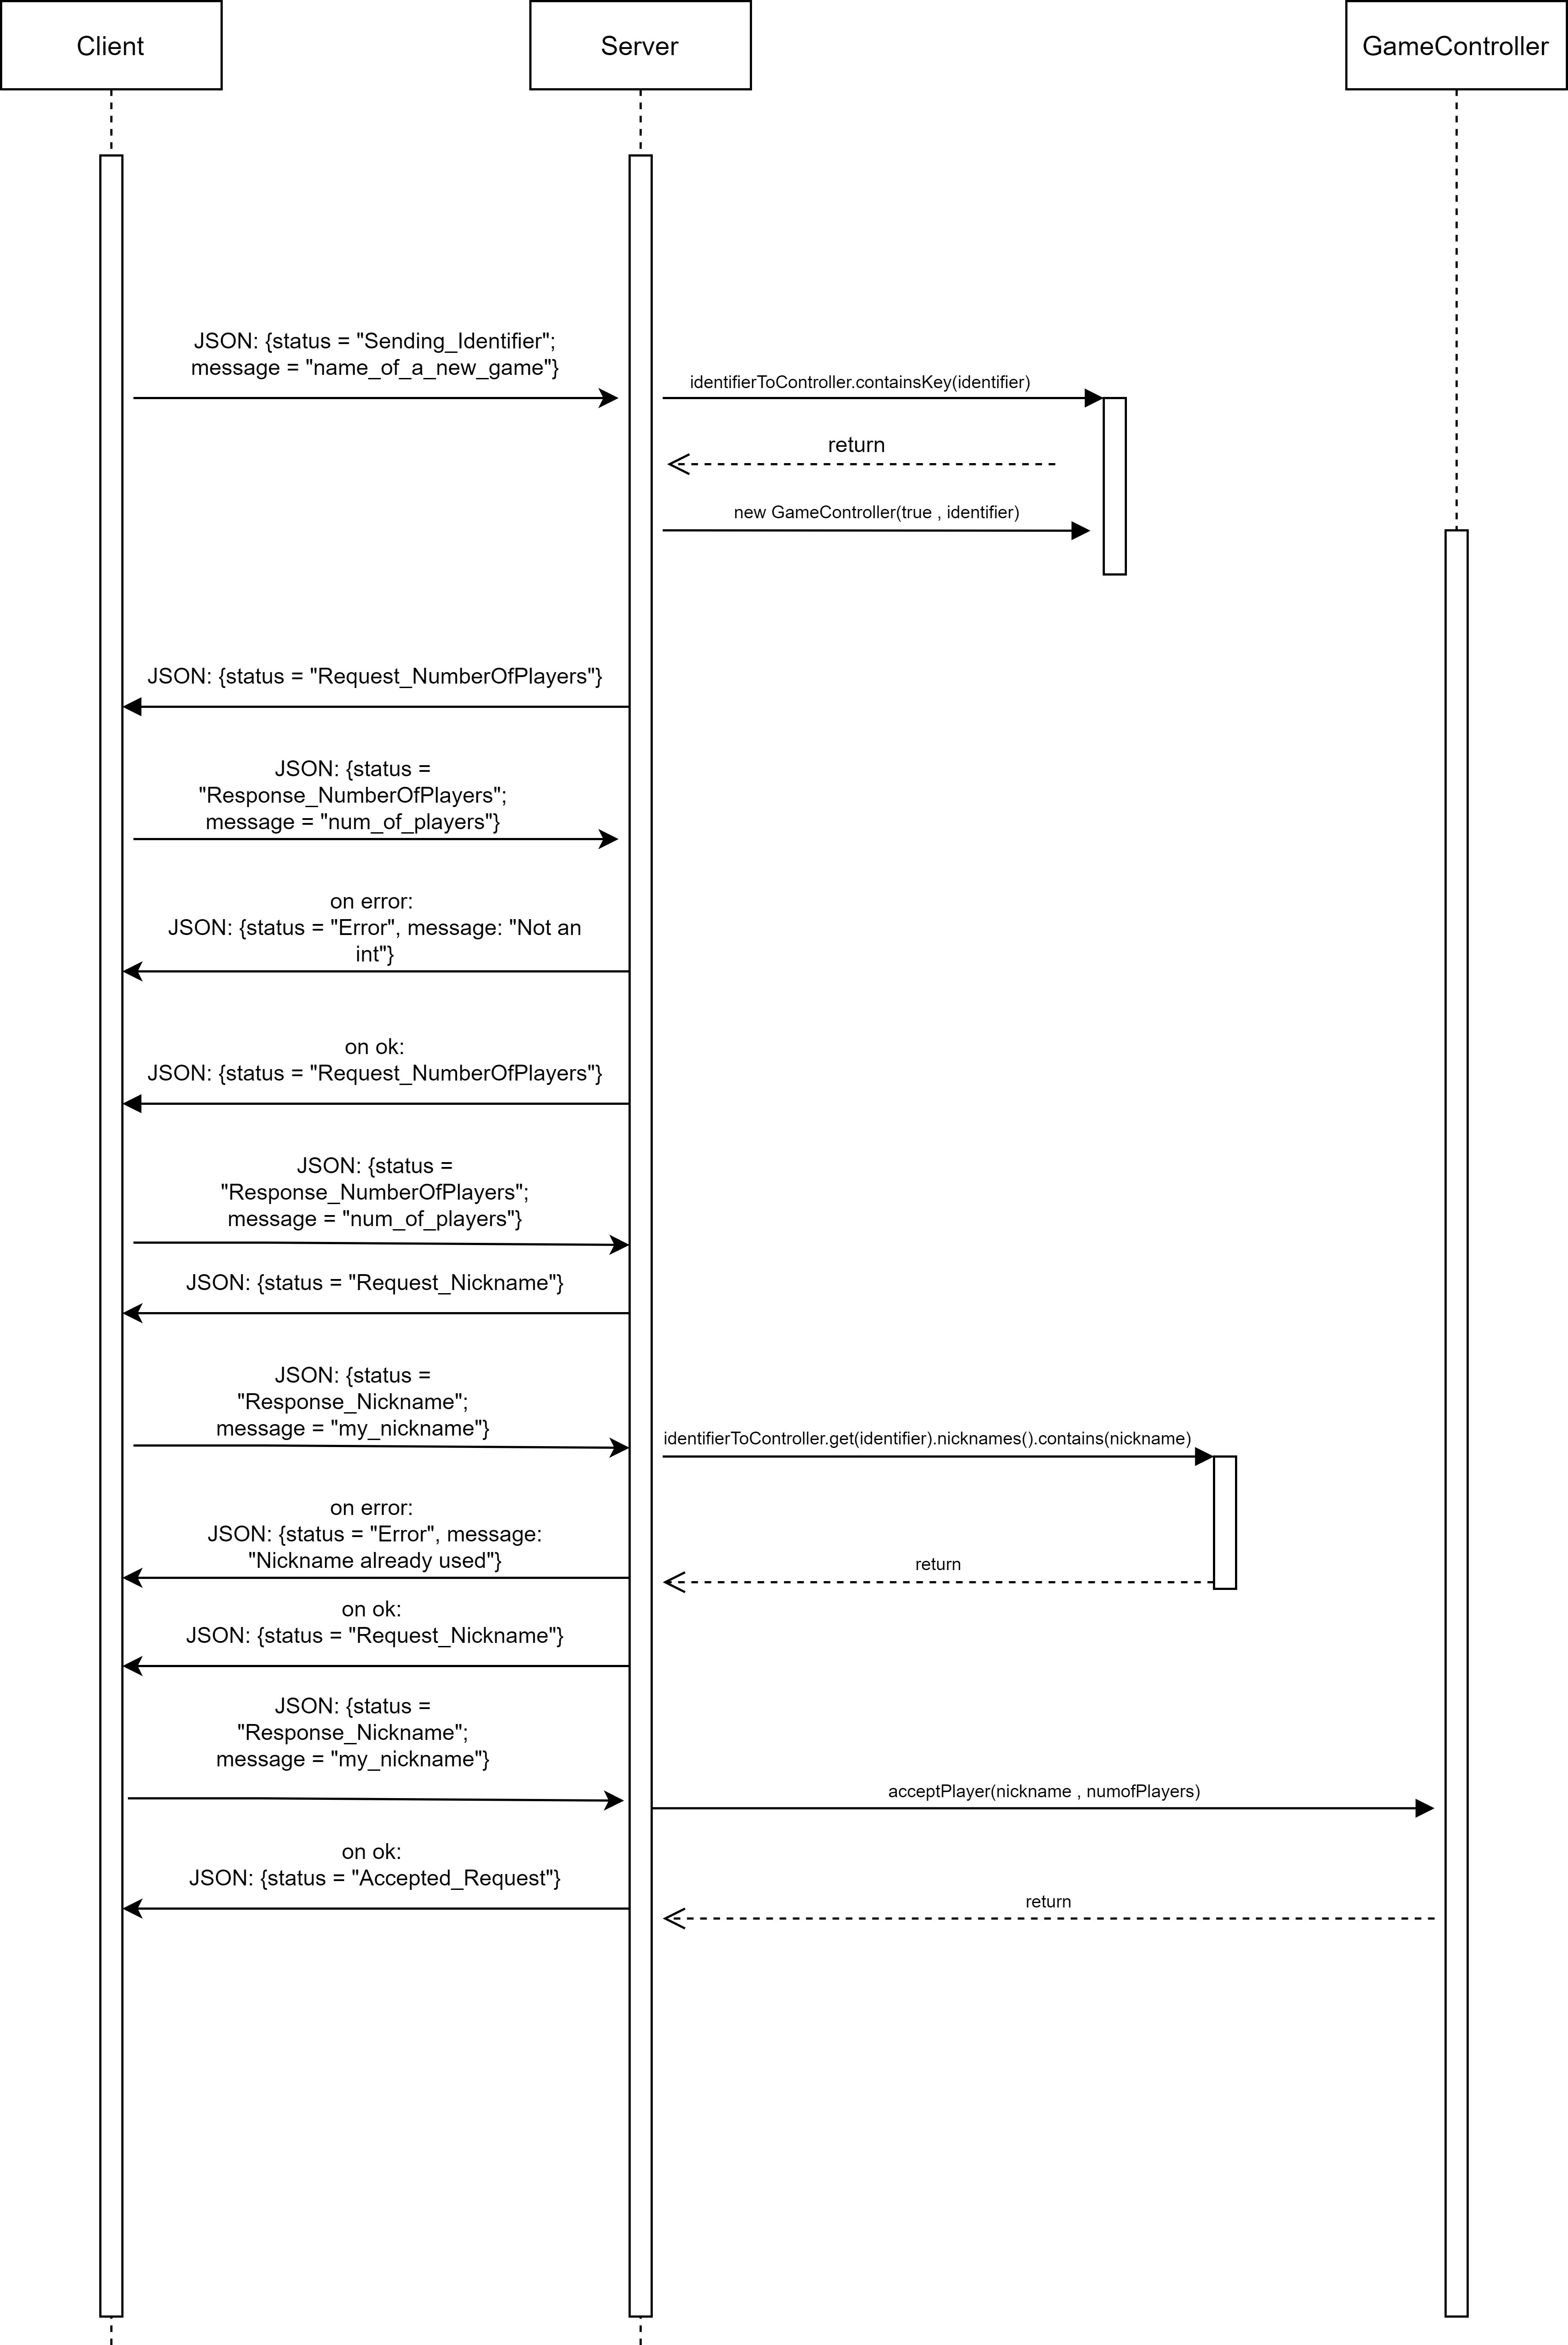
\includegraphics[height=%
    0.93\textheight]{../res/socket-1}

    \newpage

    \subsubsection{Preparazione e svolgimento del turno}

    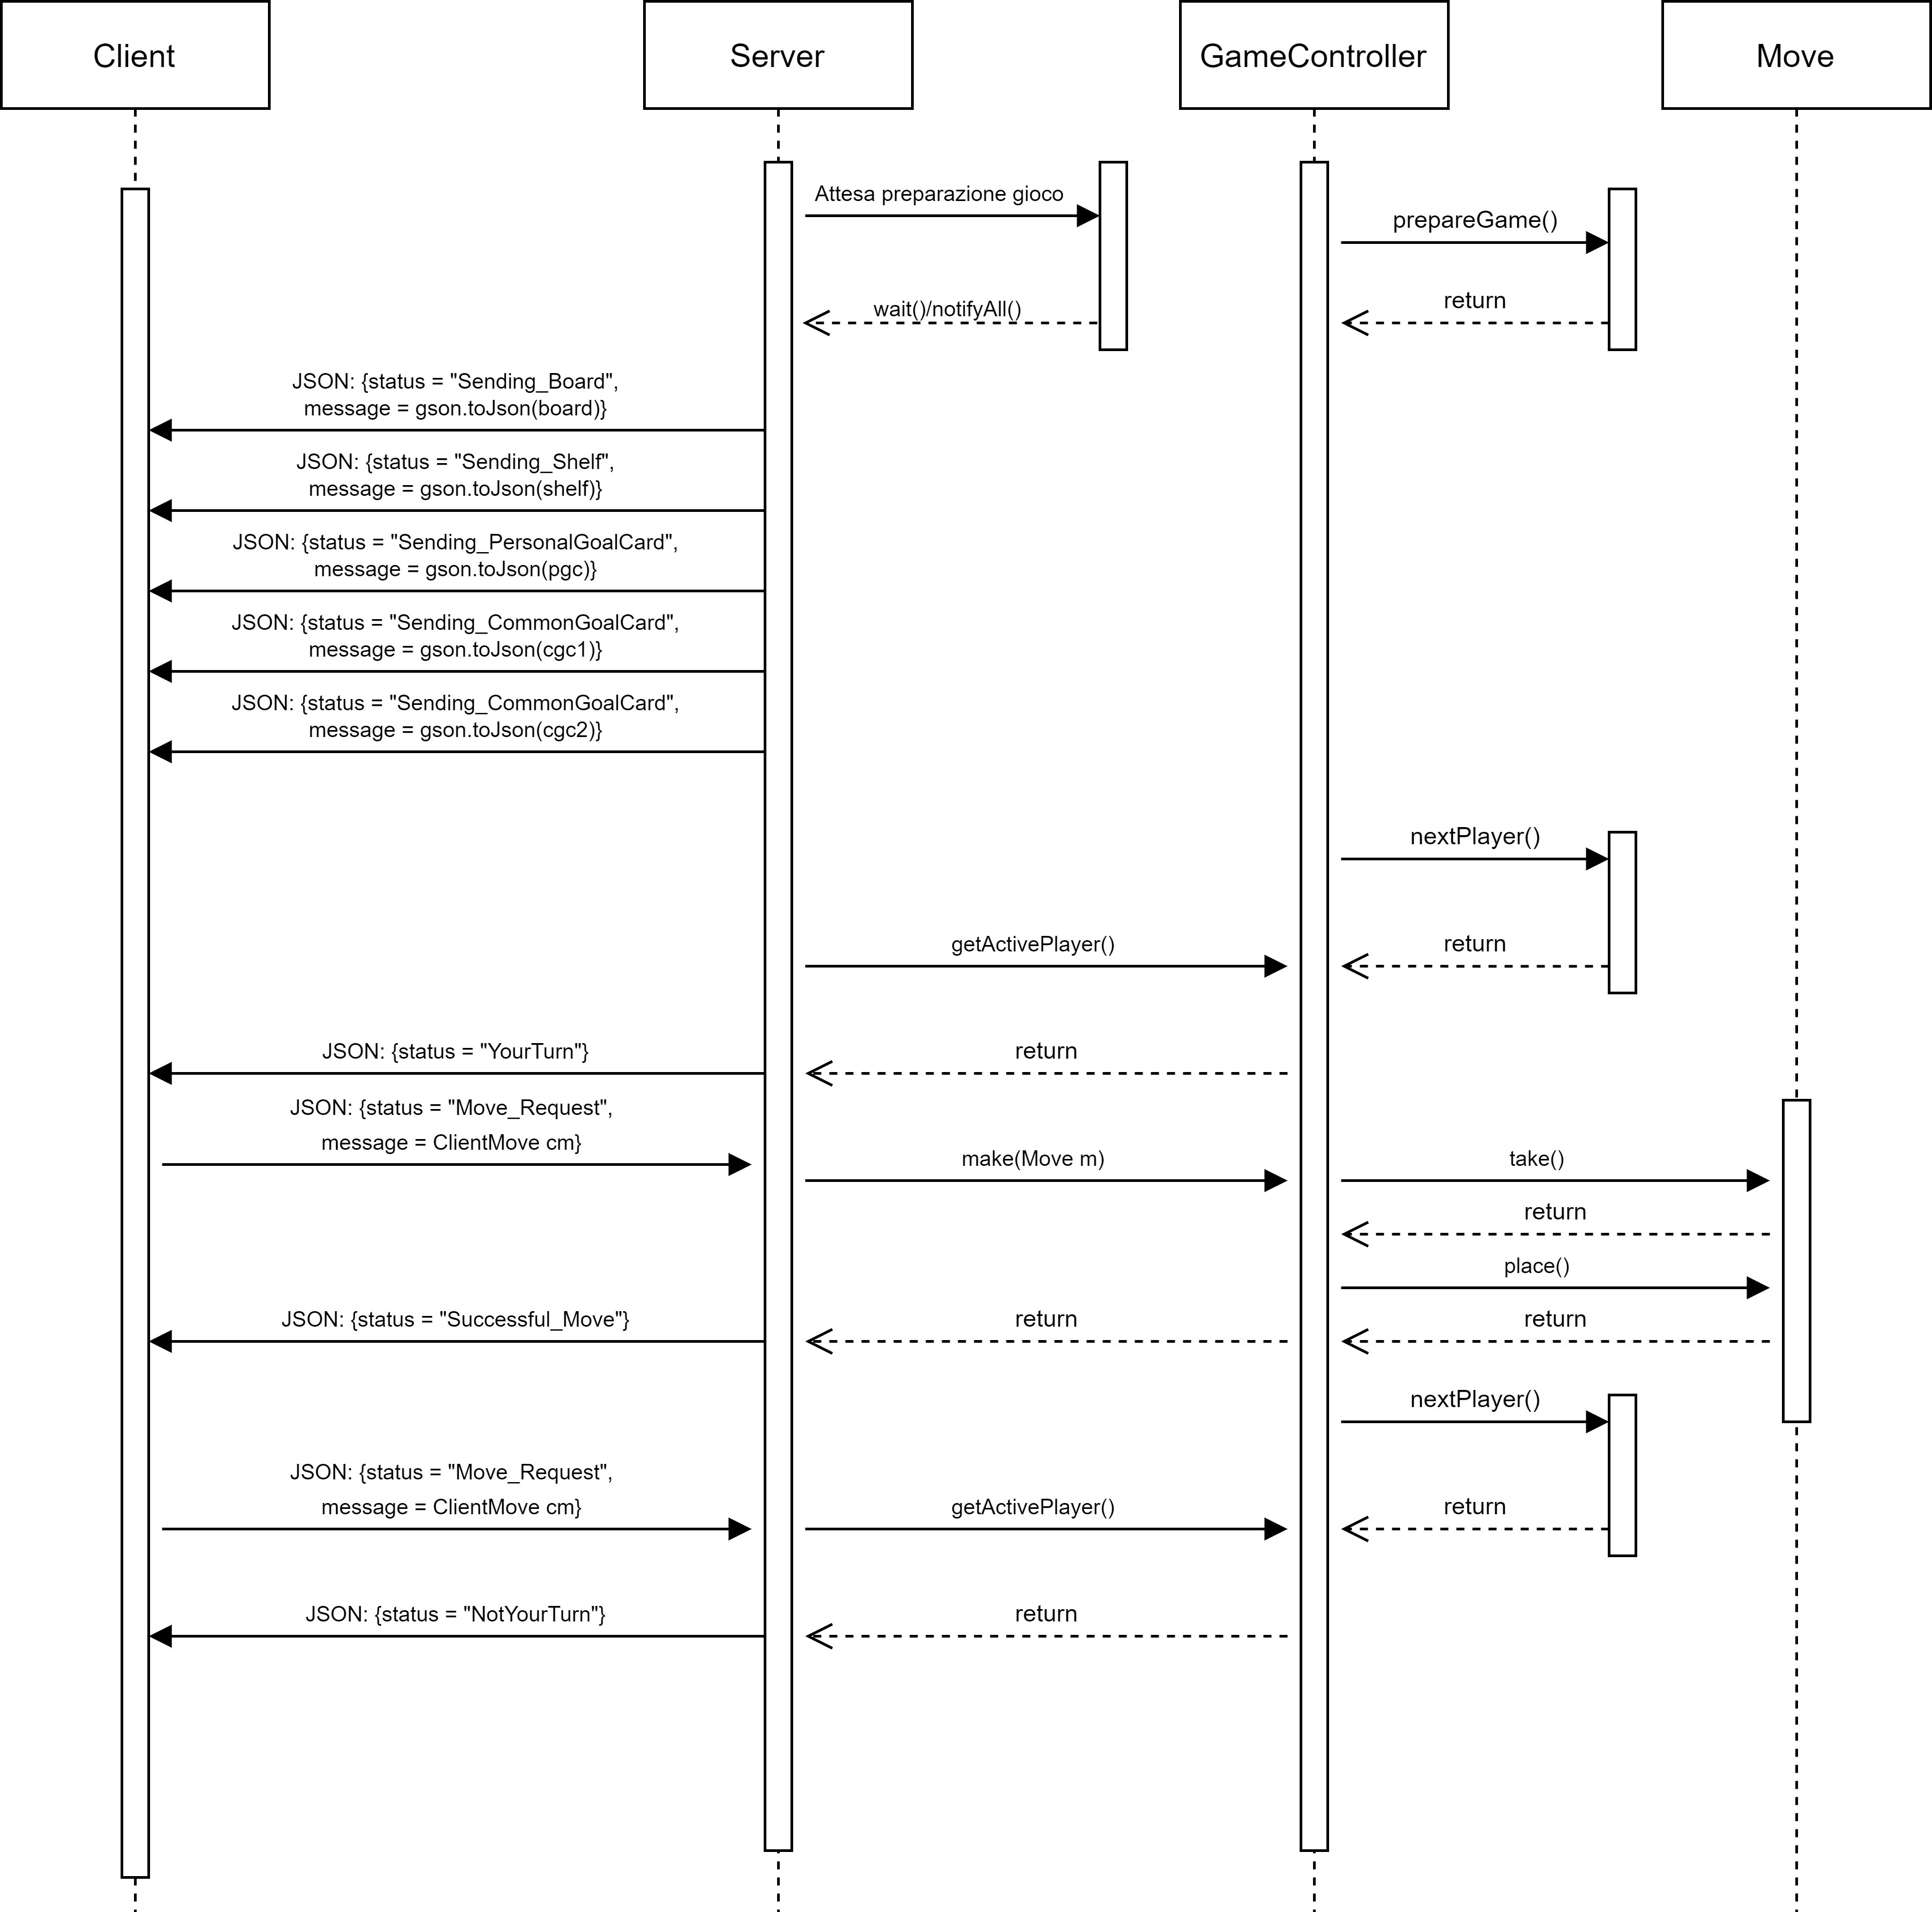
\includegraphics[height=%
    0.65\textheight]{../res/socket-2}

    \newpage

    \subsubsection{Conclusione del gioco e formulazione della classifica finale}

    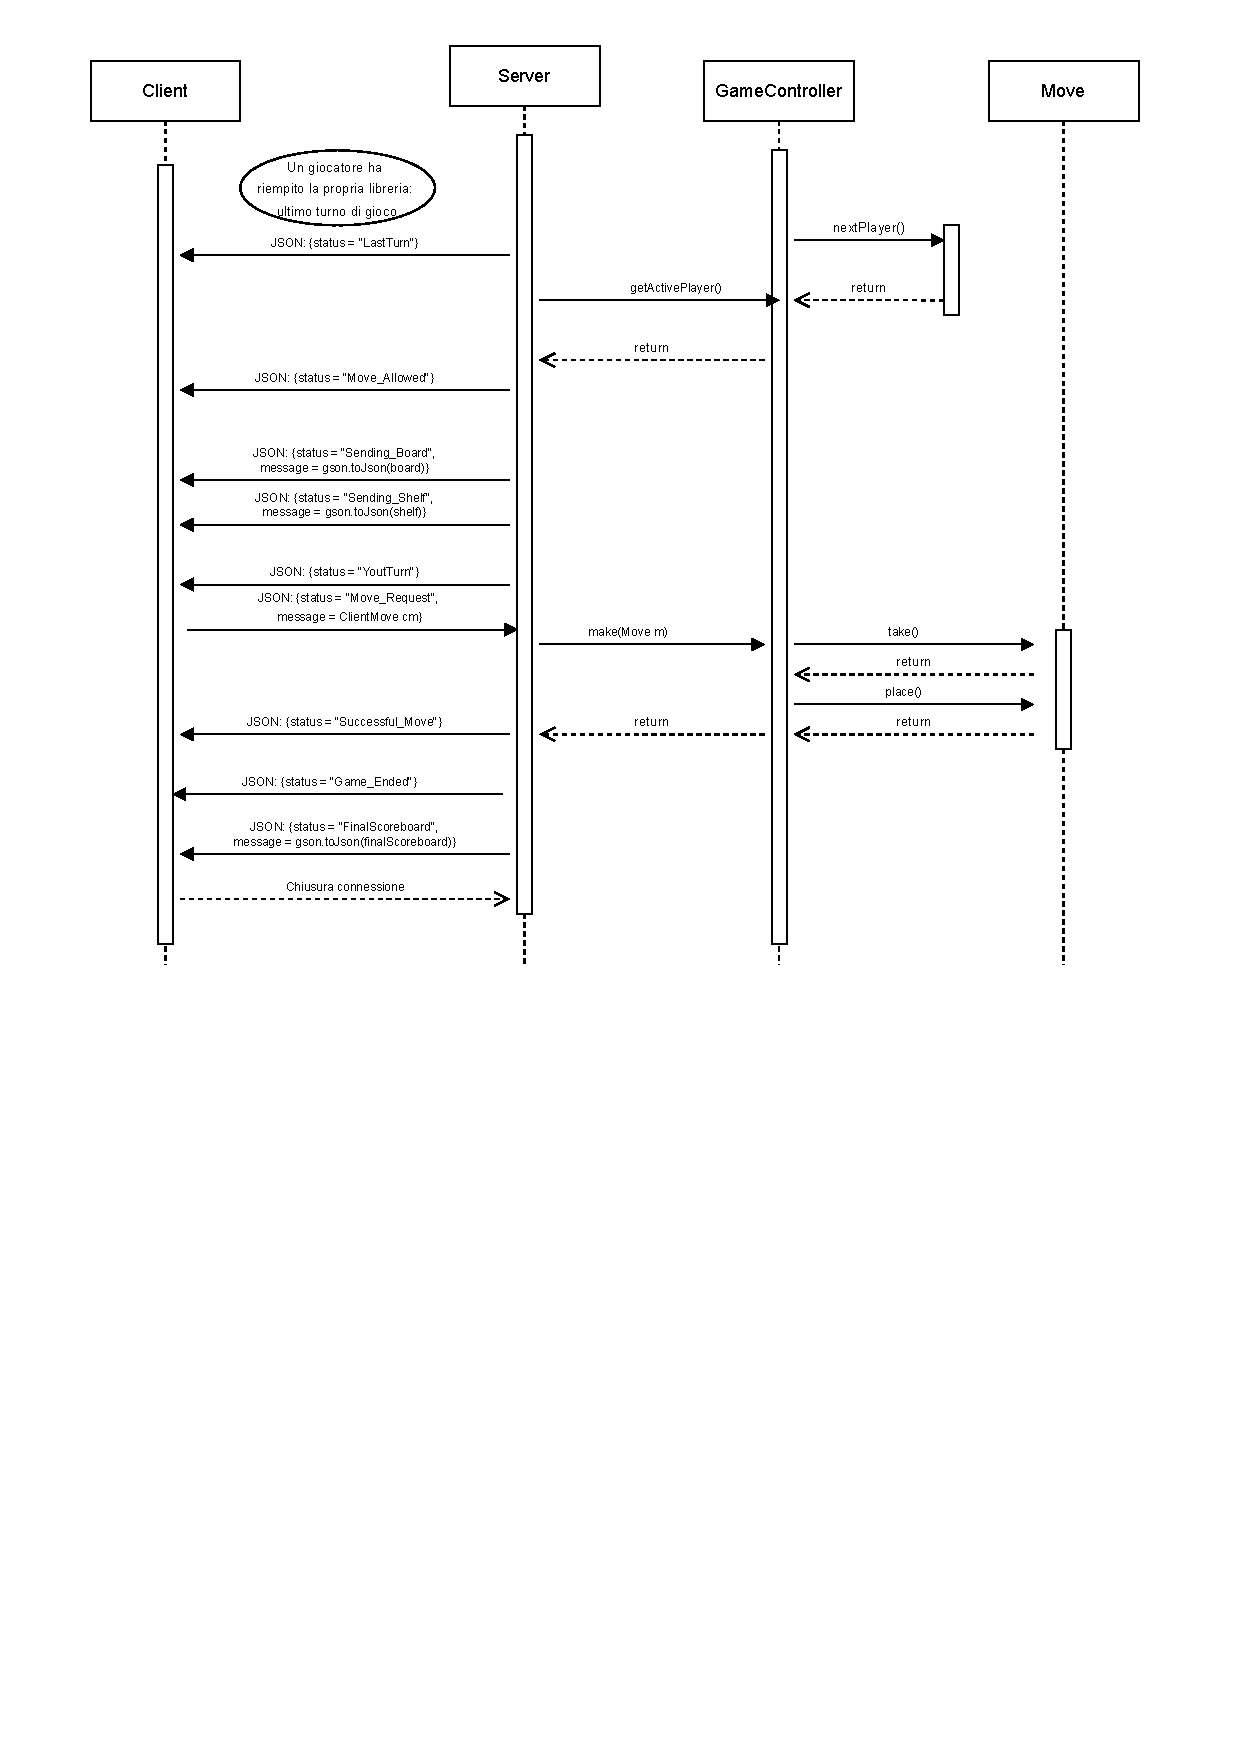
\includegraphics[height=%
    0.57\textheight]{../res/socket-3}


    \newpage


    \section{RMI}\label{sec:rmi}

    La struttura predisposta per RMI adotta numerose interfacce, attraverso cui il client fa uso dei metodi preposti alla gestione del gioco sul server.

    \smallskip

    Sono previste classi di \texttt{callback}, intermediari attraverso cui il client fornisce al server il proprio riferimento remoto, in modo che possa interagirvi,
    fornendogli i riferimenti alle interfacce che ha il diritto di utilizzare.

    \smallskip

    Sono inoltre previsti ‘‘classi di stato’’, che raccolgono i riferimenti a tali oggetti remoti e li mettono a disposizione del client.

    \subsection{Interfacce}\label{subsec:interfacce}

    Di seguito, le interfacce che il client ha a disposizione per controllare l'andamento del gioco sul server (esso implementa, naturalmente, controlli di validità).

    Tali interfacce dovranno, idealmente, comparire in ogni implementazione del client in RMI, che non ha dunque bisogno di conoscere i dettagli implementativi del modello.

    \subsubsection{Plancia di gioco}

    \begin{minted}{Java}
package it.polimi.ingsw;

import java.rmi.Remote;

public interface BoardInterface extends Remote {
    /**
     * Maximum X dimension of the board
     */
    public static final int BOARD_DIM_X = 9;
    /**
     * Maximum Y dimension of the board
     */
    public static final int BOARD_DIM_Y = 9;

    /**
     * Checks if a space is usable given coordinates
     *
     * @param x coordinate
     * @param y coordinate
     * @return usability of that space
     * @throws Exception if parameters are trying to go out of the board
     */
    public boolean isSpaceUsable(int x, int y) throws Exception;

    /**
     * Returns Object Card's type ordinal, given a Board Space
     *
     * @param x coordinate
     * @param y coordinate
     * @return the card's ordinal
     * @throws Exception if parameters are trying to go out of the board
     */
    public int getCardOrdinalFromSpace(int x, int y) throws Exception;

    /**
     * Returns Object Card's image path, given a Board Space
     *
     * @param x coordinate
     * @param y coordinate
     * @return the card's image path
     * @throws Exception if parameters are trying to go out of the board
     */
    public String getCardImageFromSpace(int x, int y) throws Exception;
}
    \end{minted}

    \newpage

    \subsubsection{Libreria personale}

    \begin{minted}{Java}
package it.polimi.ingsw;

import java.rmi.Remote;
import java.rmi.RemoteException;

public interface ShelfInterface extends Remote {
    /**
     * Maximum X dimension of the shelf
     */
    public static final int SHELF_DIM_X = 6;
    /**
     * Maximum Y dimension of the shelf
     */
    public static final int SHELF_DIM_Y = 5;

    /**
     * Returns Object Card's type ordinal in position (x, y) if valid (else -1)
     *
     * @param x coordinate
     * @param y coordinate
     * @return requested Object Card's type ordinal
     * @throws Exception if coordinates are invalid
     */
    public int getCardOrdinal(int x, int y) throws Exception;

    /**
     * Returns Object Card's image path in position (x, y) if valid (else null)
     *
     * @param x coordinate
     * @param y coordinate
     * @return the card's image path
     * @throws Exception if parameters are trying to go out of the board
     */
    public String getCardImage(int x, int y) throws Exception;

    /**
     * @return true if the Shelf is full
     */
    public boolean isFull() throws RemoteException;
}
    \end{minted}

    \newpage

    \subsubsection{Carta oggetto}

    \begin{minted}{Java}
package it.polimi.ingsw;

import java.rmi.Remote;

public interface ObjectCardInterface extends Remote {
    /**
     * This method associates an int to a letter referred to an ObjectCardType
     *
     * @param c char read from file
     * @return an int
     * @throws Exception when char doesn't match any first letter of the ObjectCardTypes
     */
    public static int getOrdinal(char c) throws Exception {
        switch (c) {
            case 'C' -> {
                return 0;
            }
            case 'B' -> {
                return 1;
            }
            case 'G' -> {
                return 2;
            }
            case 'F' -> {
                return 3;
            }
            case 'T' -> {
                return 4;
            }
            case 'P' -> {
                return 5;
            }
        }
        throw new Exception();
    }

    /**
     * Returns a char corresponding to the ordinal of a given card type.
     *
     * @param ordinal position in ObjectCardType enumeration
     * @return the corresponding char
     * @throws Exception if ordinal given does not correspond to an ObjectCardType
     */
    public static char getChar(int ordinal) throws Exception {
        switch (ordinal) {
            case 0 -> {
                return 'C';
            }
            case 1 -> {
                return 'B';
            }
            case 2 -> {
                return 'G';
            }
            case 3 -> {
                return 'F';
            }
            case 4 -> {
                return 'T';
            }
            case 5 -> {
                return 'P';
            }
        }
        throw new Exception();
    }
}
    \end{minted}

    \newpage

    \subsubsection{Carta obiettivo personale}
    \begin{minted}{Java}
package it.polimi.ingsw;

import java.rmi.Remote;
import java.rmi.RemoteException;

public interface PersonalGoalCardInterface extends Remote {
    /**
     * Limit of Personal Goal Cards.
     */
    public static final int LIMIT = 12;

    /**
     * Getter method for Personal Goal Card
     *
     * @return type of the card
     */
    public int getType() throws RemoteException;

    /**
     * getter method
     *
     * @param x coordinate
     * @param y coordinate
     * @return ordinal of ObjectCardType or -1 if the card is empty
     * @throws Exception if coordinates are invalid
     */
    public int getOrdinal(int x, int y) throws Exception;
}
    \end{minted}

    \newpage

    \subsubsection{Carta obiettivo comune}

    \begin{minted}{Java}
package it.polimi.ingsw;

import java.rmi.Remote;
import java.rmi.RemoteException;

public interface CommonGoalCardInterface extends Remote {
    /**
     * Limit of Common Goal Cards.
     */
    public static final int LIMIT = 12;

    /**
     * This method returns the textual description of the pattern that the player has to achieve, in order
     * to gain points.
     *
     * @return String: textual description of the pattern
     */
    public String getDescription() throws RemoteException;
}
    \end{minted}

    \newpage

    \subsubsection{Intermediario delle mosse}
    Per ogni client, esso conosce i riferimenti al suo Controller di gioco e
    alla relativa plancia e carte obiettivo comune e personale, nonché alla libreria personale del giocatore.

    \begin{minted}{Java}
package it.polimi.ingsw;

import java.rmi.Remote;
import java.rmi.RemoteException;
import java.util.List;

public interface MoveIntermediateInterface extends Remote {
    /**
     * Move parameters
     *
     * @param x      list of coordinates (x)
     * @param y      list of coordinates (y)
     * @param column in the Player's shelf
     */
    public void setParameters(List<Integer> x, List<Integer> y, int column) throws RemoteException;

    /**
     * Move's creation and confirmation
     *
     * @return validity of the move
     * @throws Exception related to Shelf and Board management
     */
    public boolean make() throws Exception;

    /**
     * @return validity of the last move
     */
    public boolean isLastMoveValidated() throws RemoteException;
}
    \end{minted}

    \newpage

    \subsubsection{Stato del client}
    Aggregato: contiene i riferimenti alle interfacce cui il client ha diritto di accesso durante il gioco.

    Si noti che il client ha accesso alle sole interfacce e non conosce i dettagli di implementazione del modello.

    \smallskip

    Per favorire la leggibilità, si omette la JavaDoc di alcuni metodi (la cui funzione è ritenuta chiara dal contesto).

    \begin{minted}{Java}
package it.polimi.ingsw;

import java.rmi.Remote;
import java.rmi.RemoteException;
import java.util.List;

public interface ClientStatusInterface extends Remote {
    public Status getStatus() throws RemoteException;

    public boolean setStatus(Status status) throws RemoteException;

    public String getIdentifier() throws RemoteException;

    public void setIdentifier(String identifier) throws RemoteException;

    public String getNickname() throws RemoteException;

    public void setNickname(String nickname) throws RemoteException;

    /**
     * Aggregate setter for Game initial parameters
     *
     * @param board Game's board
     * @param shelf Player's shelf
     * @param mi    Move Intermediate for the client
     */
    public void setGameParameters(BoardInterface board, ShelfInterface shelf, MoveIntermediateInterface mi) throws RemoteException;

    public BoardInterface getBoard() throws RemoteException;

    public ShelfInterface getShelf() throws RemoteException;

    public PersonalGoalCardInterface getPersonalGoalCard() throws RemoteException;

    public List<CommonGoalCardInterface> getCommonGoalCard() throws RemoteException;

    public void setCards(PersonalGoalCardInterface pgCard, List<CommonGoalCardInterface> cgCard) throws RemoteException;

    public MoveIntermediateInterface getMoveIntermediate() throws RemoteException;

    public String getCurrentPlayer() throws RemoteException;

    public void setCurrentPlayer(String currentPlayer) throws RemoteException;

    public ScoreBoardInterface getScoreBoard() throws RemoteException;

    public void setScoreBoard(ScoreBoardInterface sci) throws RemoteException;
}
    \end{minted}

    \newpage

    \subsubsection{Intermediario dello stato}

    Interfaccia di \texttt{callback} per il server.

    Il client fornisce al server un riferimento alla propria implementazione del gestore di stato, che si occupa di far evolvere il client.

    Il server usa tale riferimento per comunicare l'evoluzione al client ed invitarlo a svolgere le azioni di gestione delle fasi di gioco.

    \begin{minted}{Java}
package it.polimi.ingsw;

import java.rmi.Remote;
import java.rmi.RemoteException;

public interface StatusIntermediateInterface extends Remote {
    /**
     * Setter for Client Status Object
     * It makes the server manage Game's evolution
     *
     * @param csi Interface for the Client Status
     * @throws RemoteException      related to RMI
     * @throws InterruptedException related to Thread management
     */
    public void setIntermediate(ClientStatusInterface csi) throws RemoteException, InterruptedException;
}
    \end{minted}

    \newpage

    \subsubsection{RMI Controller}
    Livello di astrazione al controller: fornisce al client i metodi necessari per la gestione delle fasi iniziali (ammissione e creazione nuove partite).

    Si rende necessario per la gestione di partite multiple.

    Sono implementati stringenti controlli di integrità relativamente all'accesso al Controller e al Modello sottostanti.

    \begin{minted}{Java}
package it.polimi.ingsw;

import java.rmi.Remote;
import java.rmi.RemoteException;

public interface RMIControllerInterface extends Remote {
    /**
     * @param identifier Game's identifier
     * @return whether the identifier exists
     */
    public boolean identifierExists(String identifier) throws RemoteException;

    /**
     * @param identifier Game's identifier
     * @param nickname   Player's nickname
     * @return whether the nickname exists in the given Game's identifier
     */
    public boolean nicknameExists(String identifier, String nickname) throws RemoteException;

    /**
     * Creates a game using the corresponding identifier
     *
     * @param identifier Game's identifier
     * @return true if the Game have been correctly created
     */
    public boolean createGame(String identifier) throws RemoteException;

    /**
     * Admission phase
     *
     * @param identifier Game's identifier
     * @param nickname   Player's nickname
     * @param maxPlayers Maximum number of players for the game
     *                   used only if the first player is being accepted to the game.
     *                   It is ignored otherwise.
     * @return true if the admission process have been correctly completed
     * @throws Exception related to Model management
     */
    public boolean acceptPlayer(String identifier, String nickname, int maxPlayers) throws Exception;
}
    \end{minted}

    \newpage

    \subsubsection{Classifica finale}
    Mappa ordinata che associa i giocatori (con il loro nickname) al loro punteggio.

    \begin{minted}{Java}
package it.polimi.ingsw;

import java.rmi.Remote;
import java.rmi.RemoteException;
import java.util.Map;

public interface ScoreBoardInterface extends Remote {
    /**
     * Getter for the final Scoreboard sorted Map
     *
     * @return final Scoreboard
     */
    public Map<String, Integer> getScoreBoard() throws RemoteException;
}
    \end{minted}

    \newpage

    \subsection{Diagrammi di sequenza}\label{subsec:diagrammi-di-sequenza2}

    \subsubsection{Accesso, selezione e ammissione al gioco}

    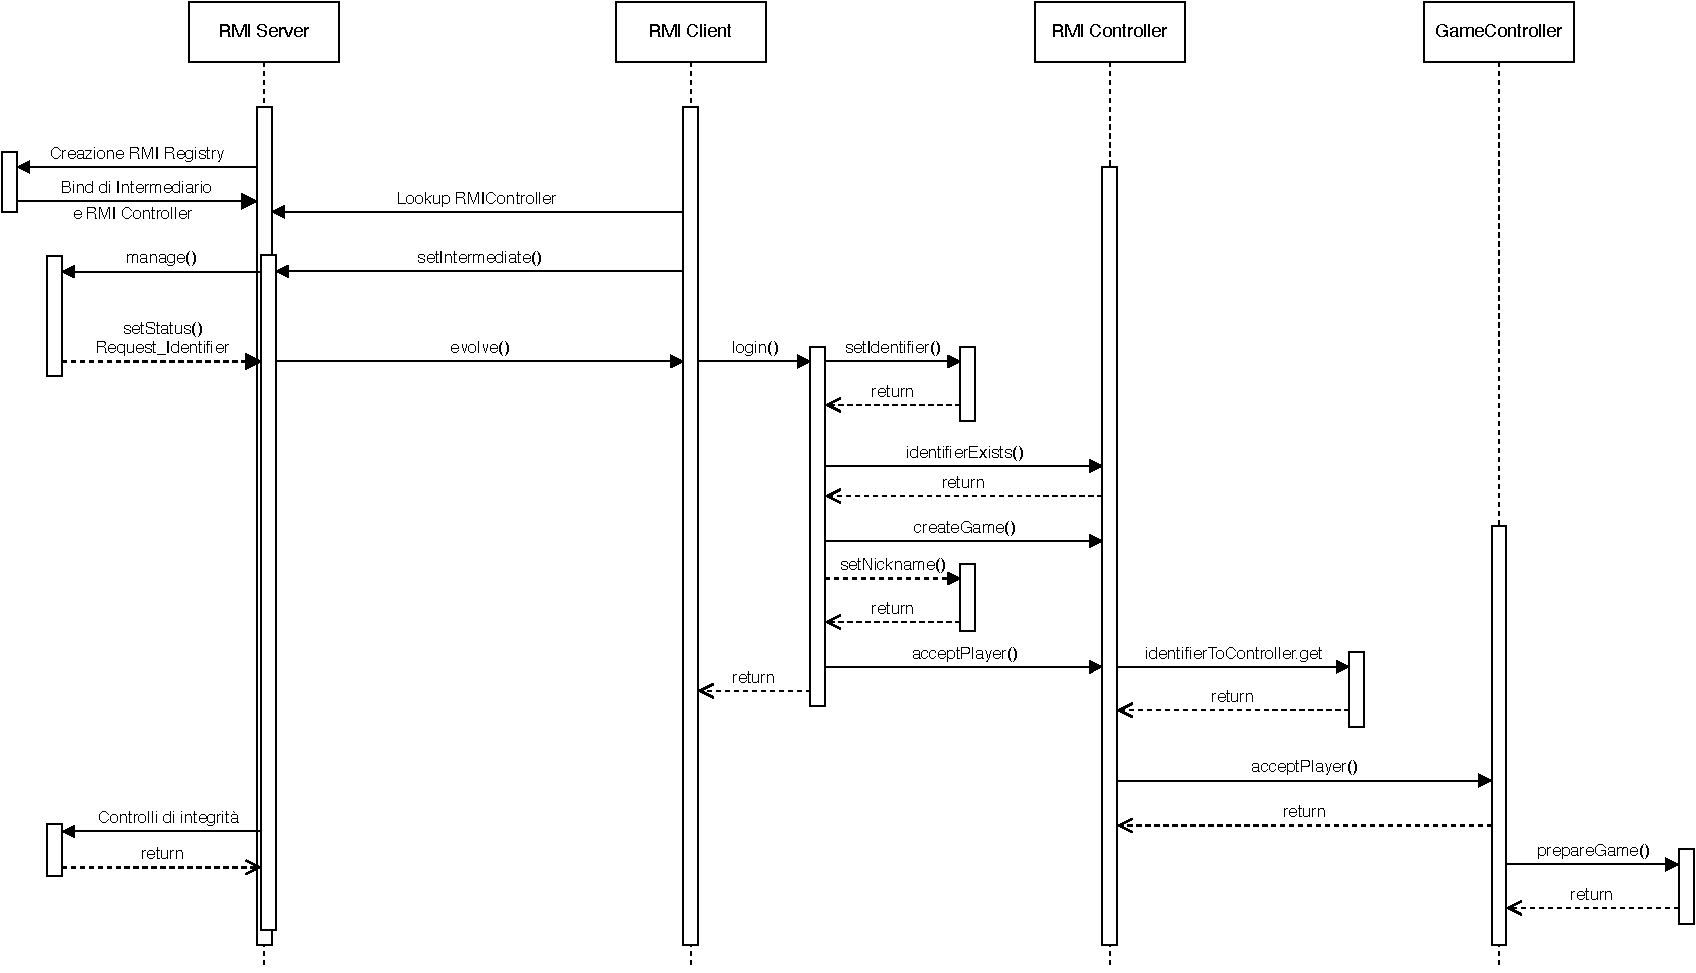
\includegraphics[height=%
    0.4\textheight]{../res/rmi-1}

    \newpage

    \subsubsection{Due mosse di esempio}

    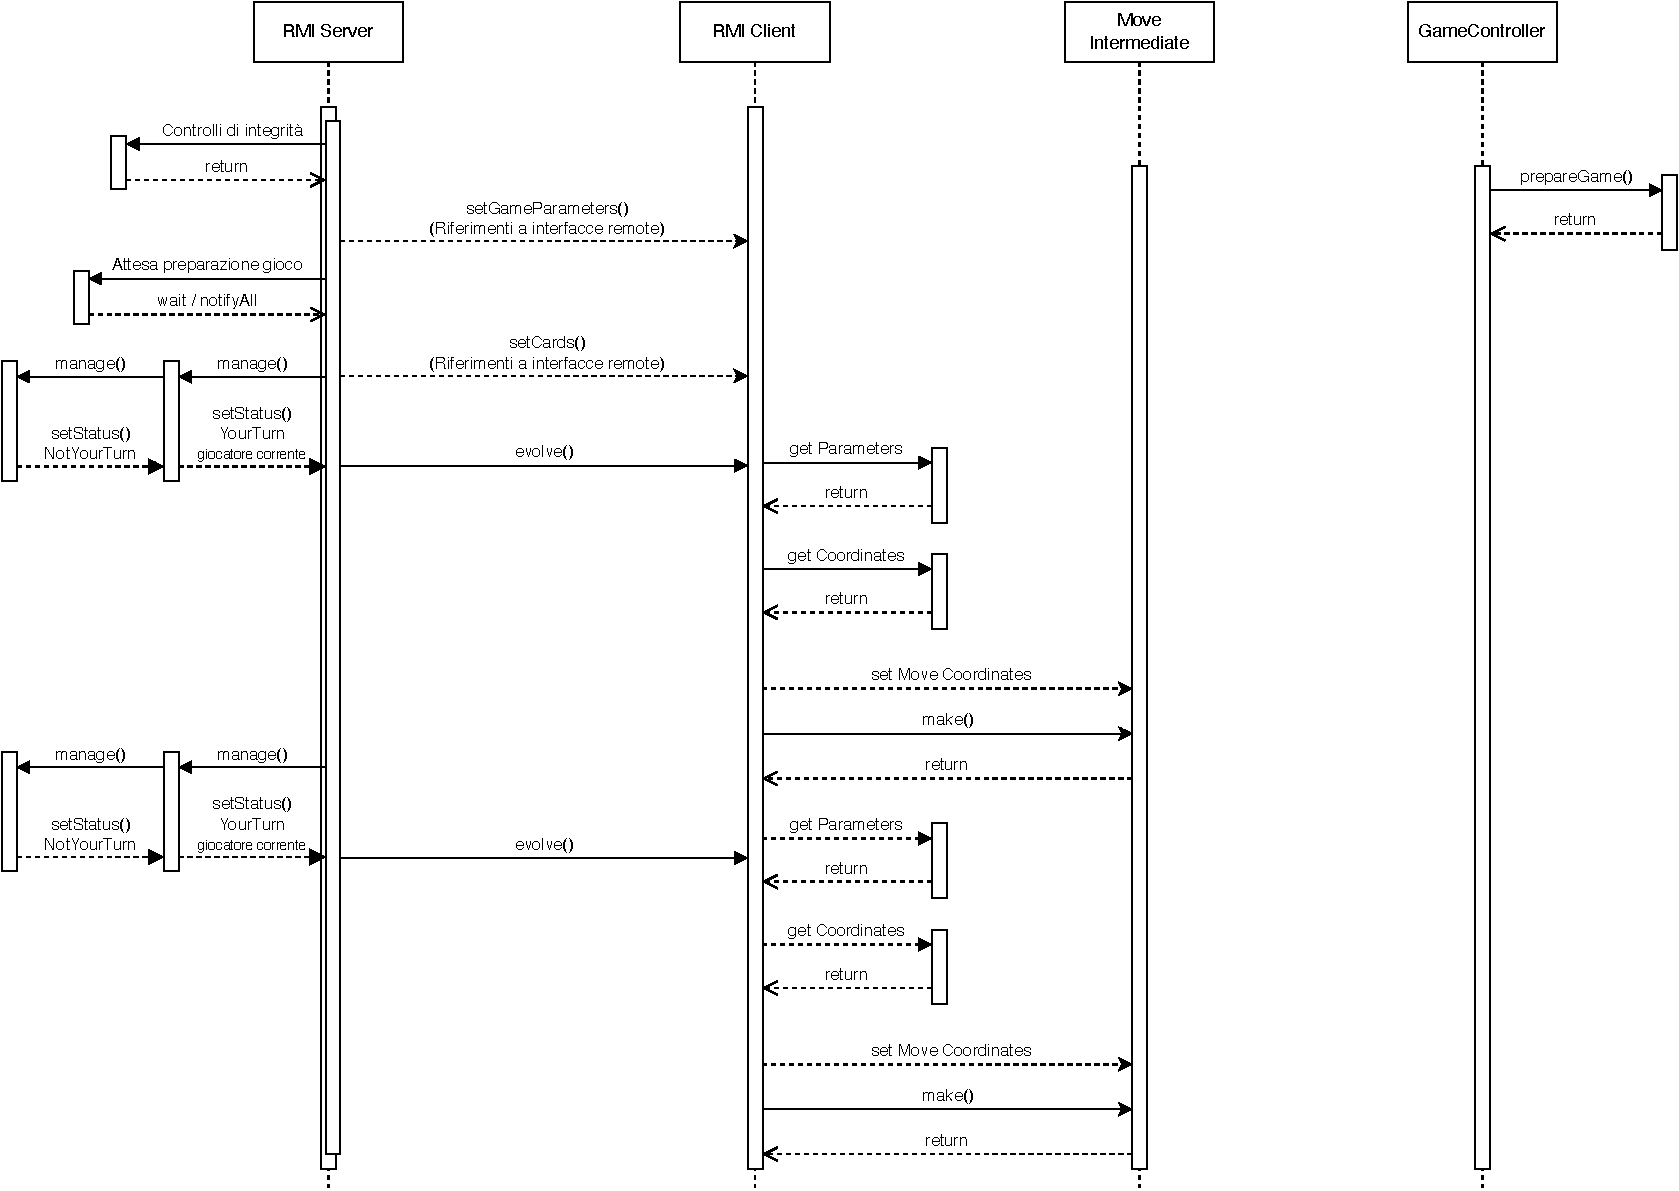
\includegraphics[height=%
    0.48\textheight]{../res/rmi-2}

    \newpage

    \subsubsection{Conclusione del gioco e formulazione della classifica finale}

    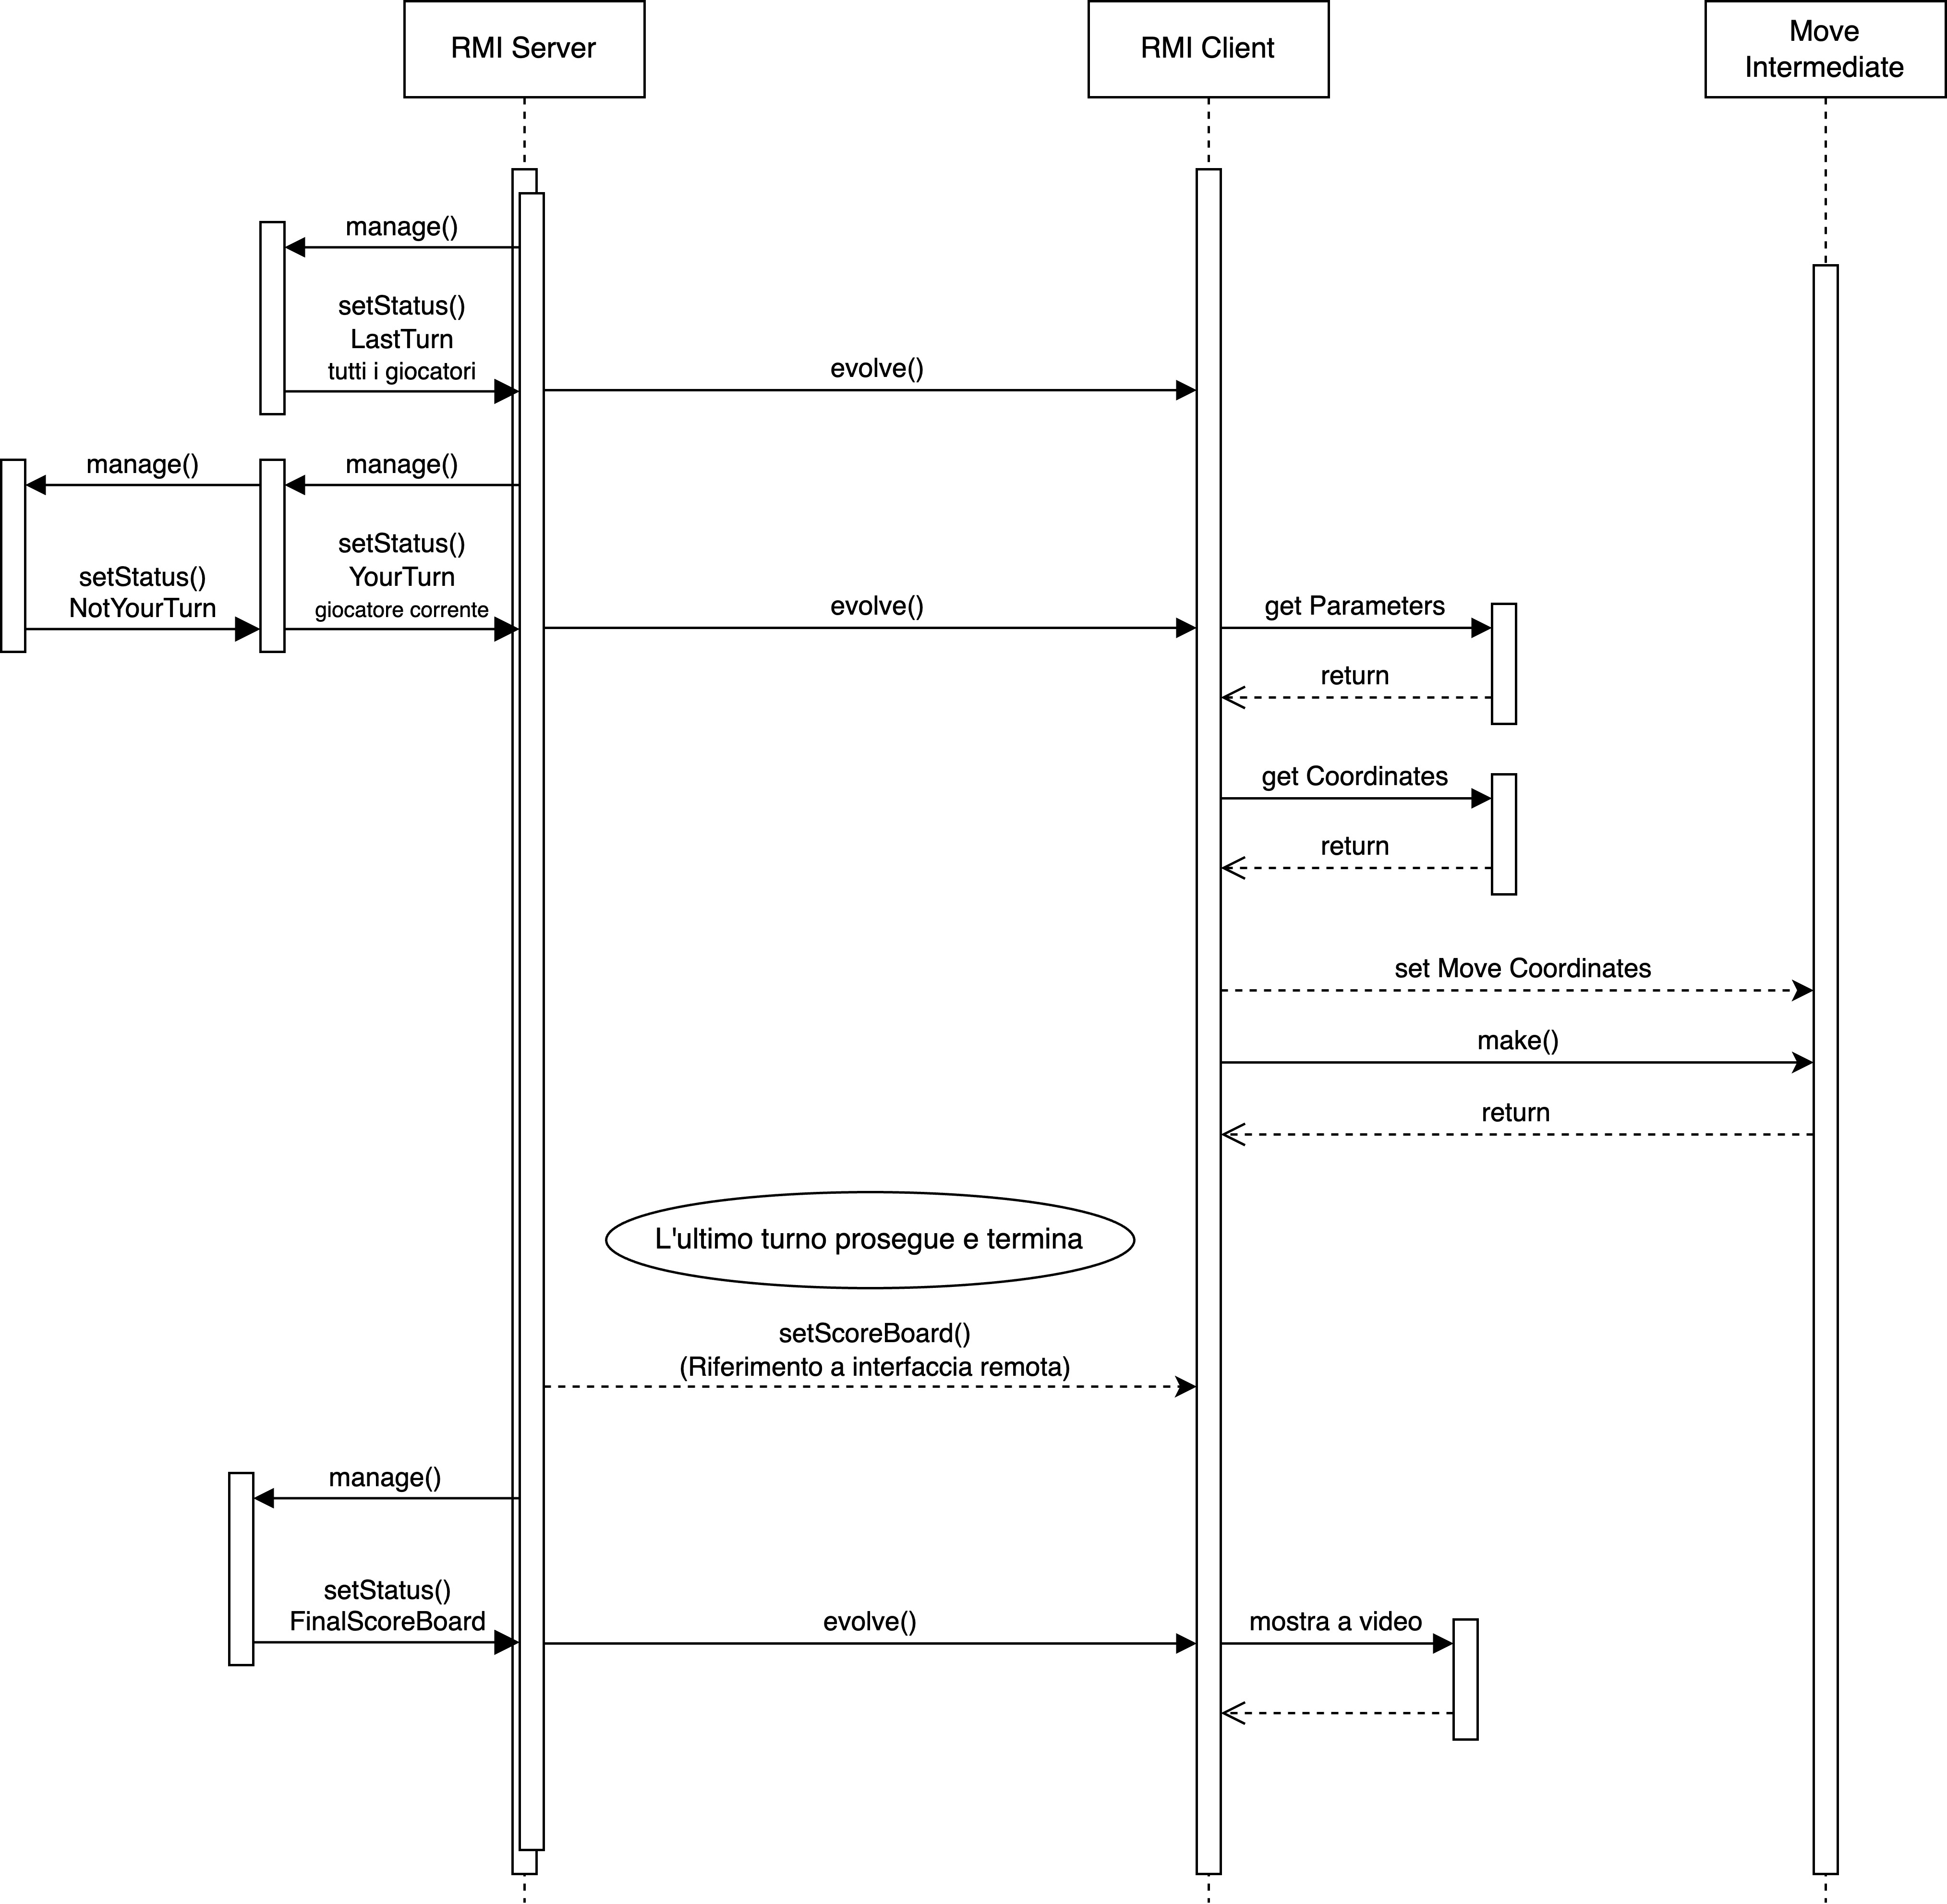
\includegraphics[height=%
    0.6\textheight]{../res/rmi-3}

    \newpage
\end{document}